\begin{figure}[th]
\caption{Various Height Cutoffs for California \label{fig:caliclusters}}
\begin{tabular}{cc}
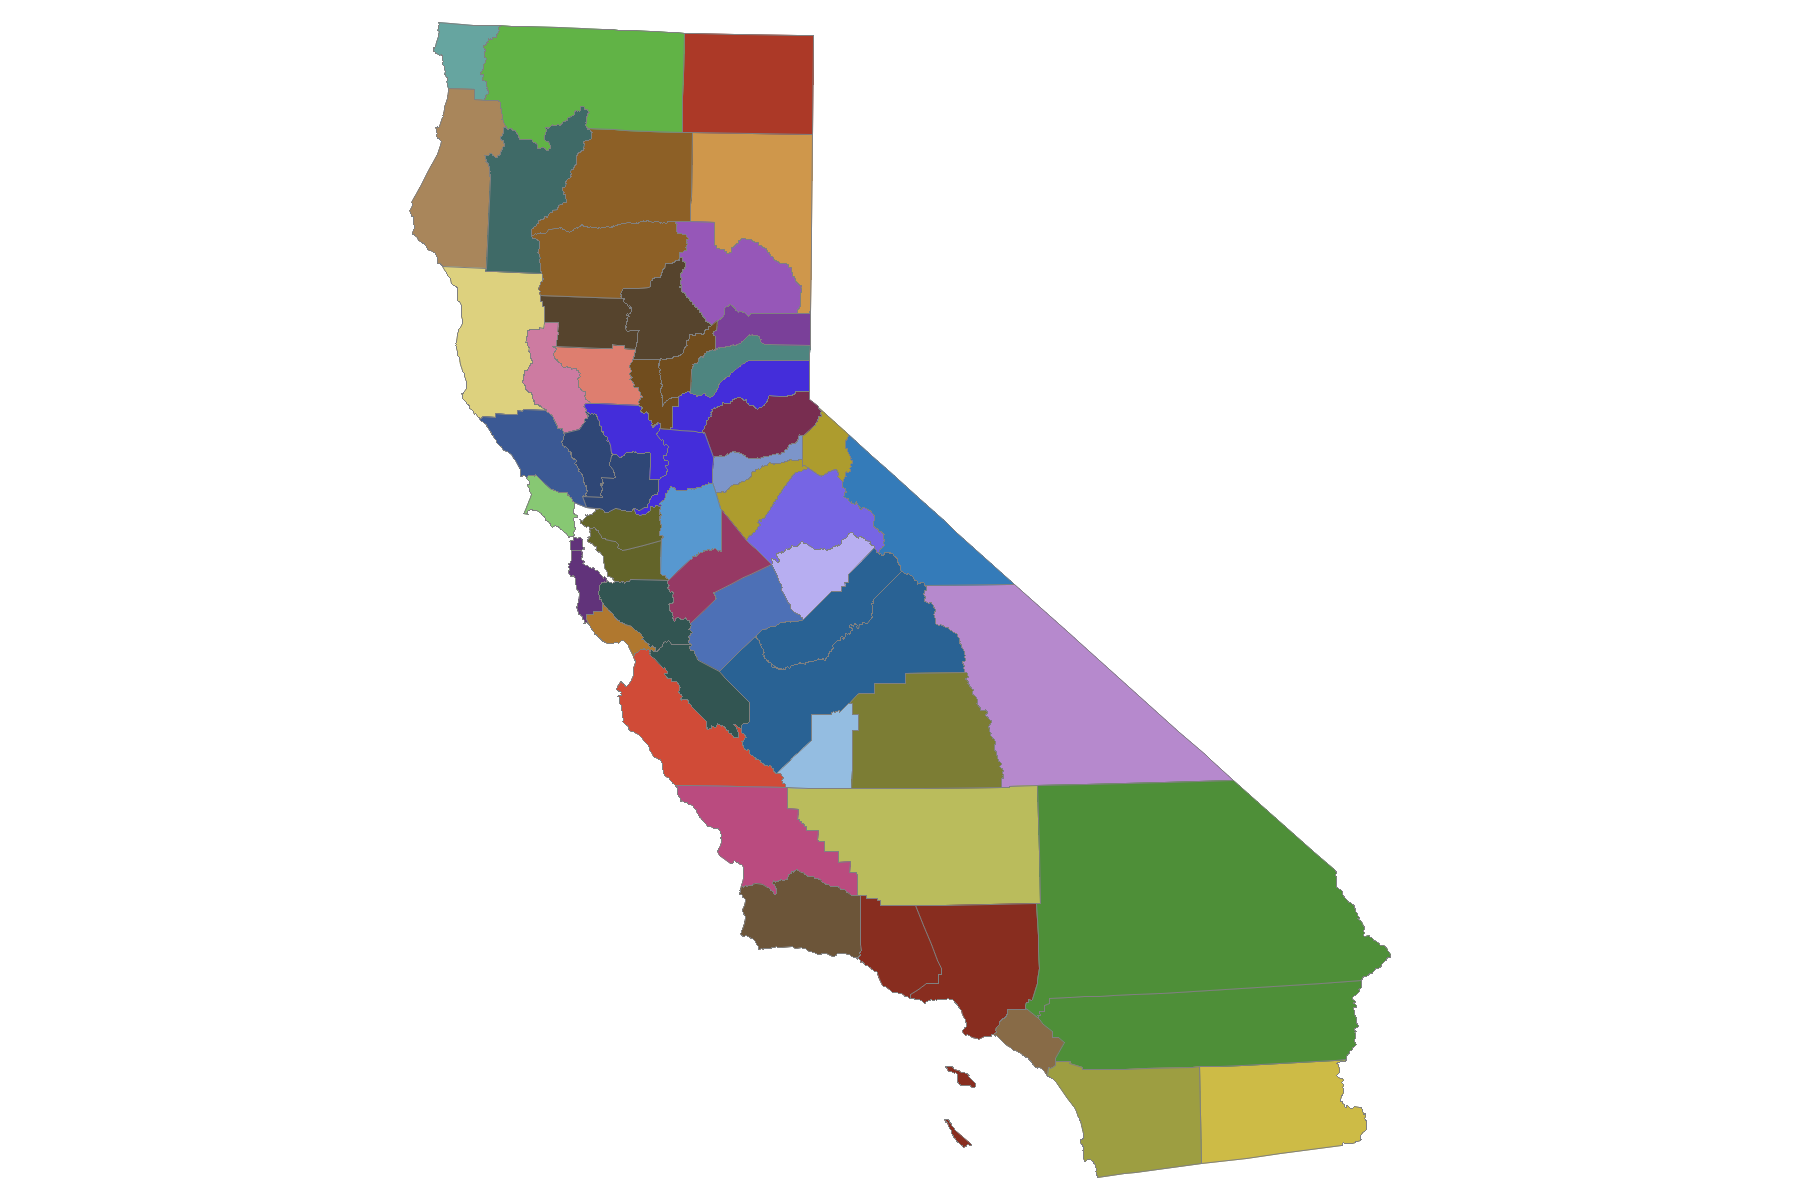
\includegraphics[scale=0.1]{./figures/insetmaps/california_clustermap_800_inset6.png} & 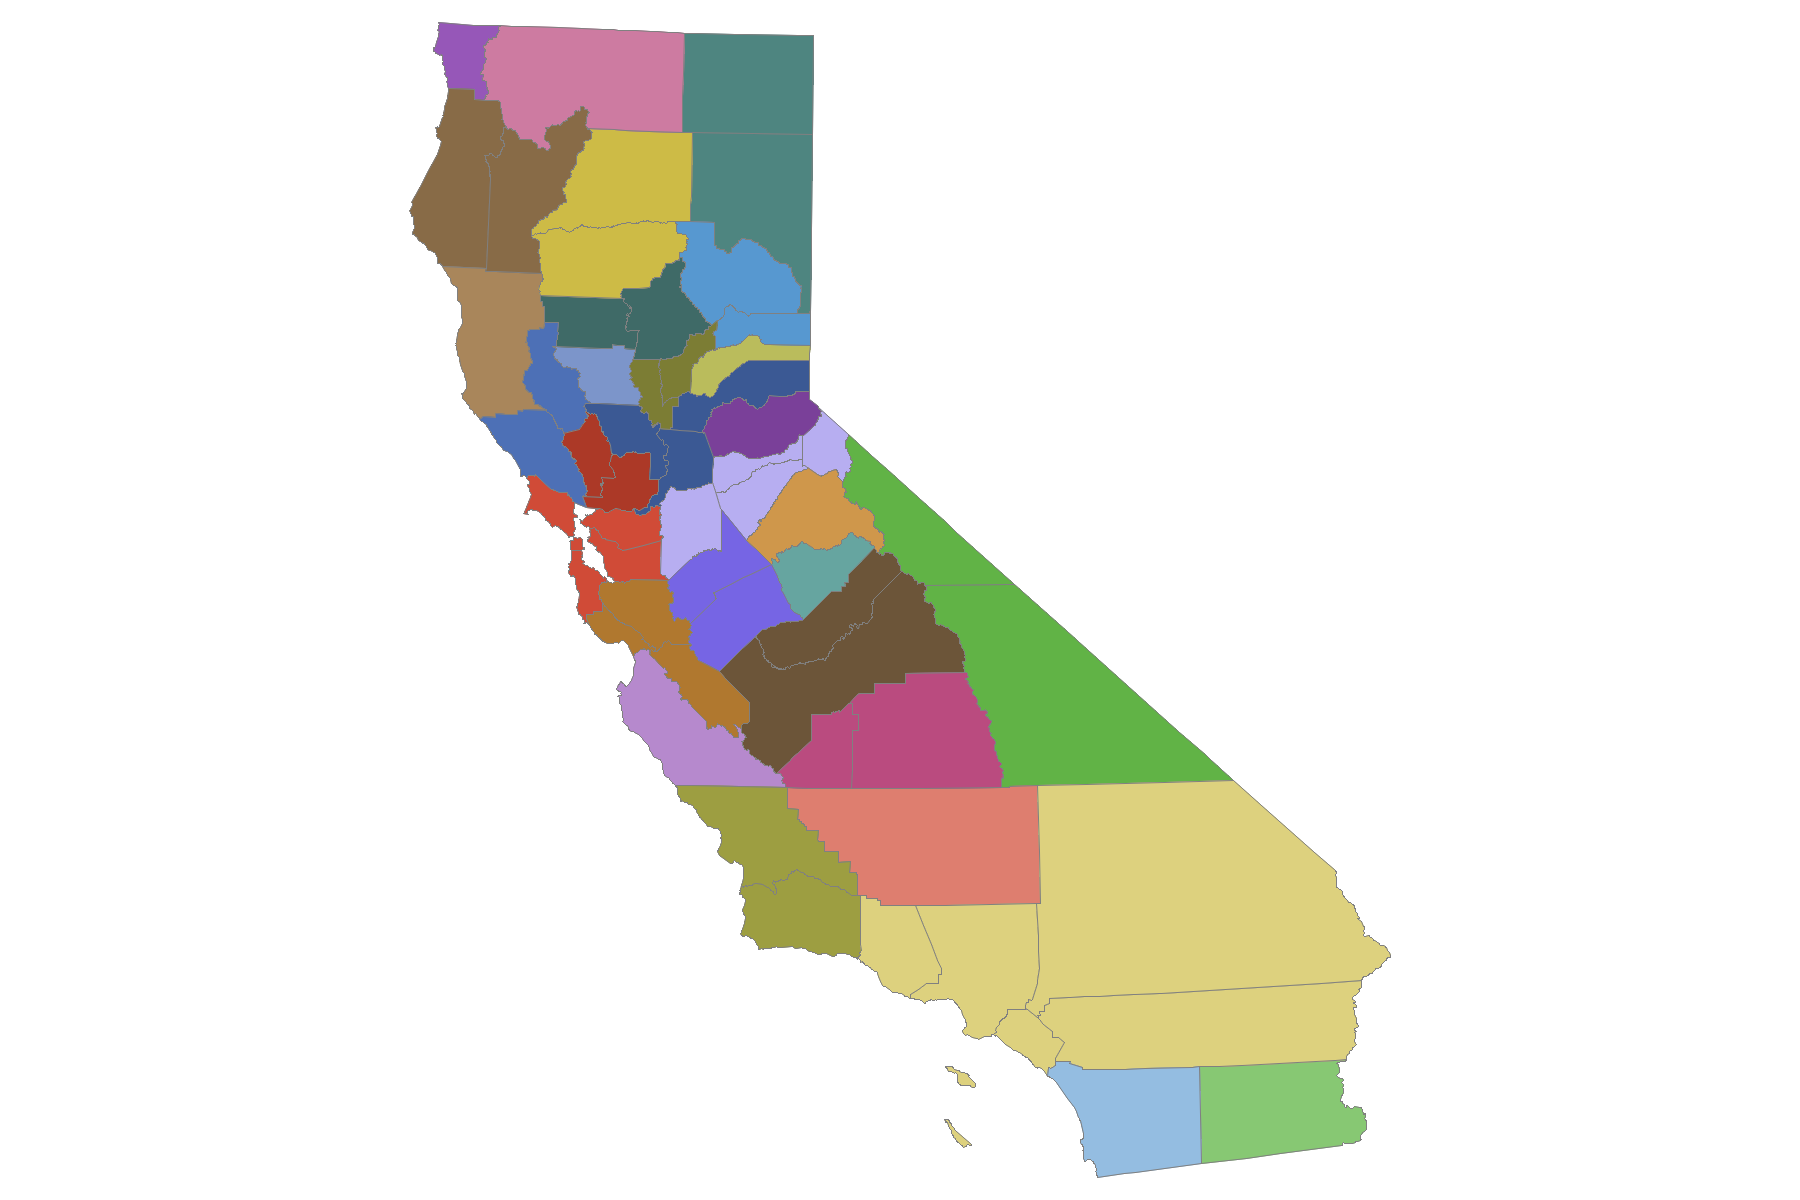
\includegraphics[scale=0.1]{./figures/insetmaps/california_clustermap_880_inset6.png} \\
Height = 0.8 & Height = 0.88 \\
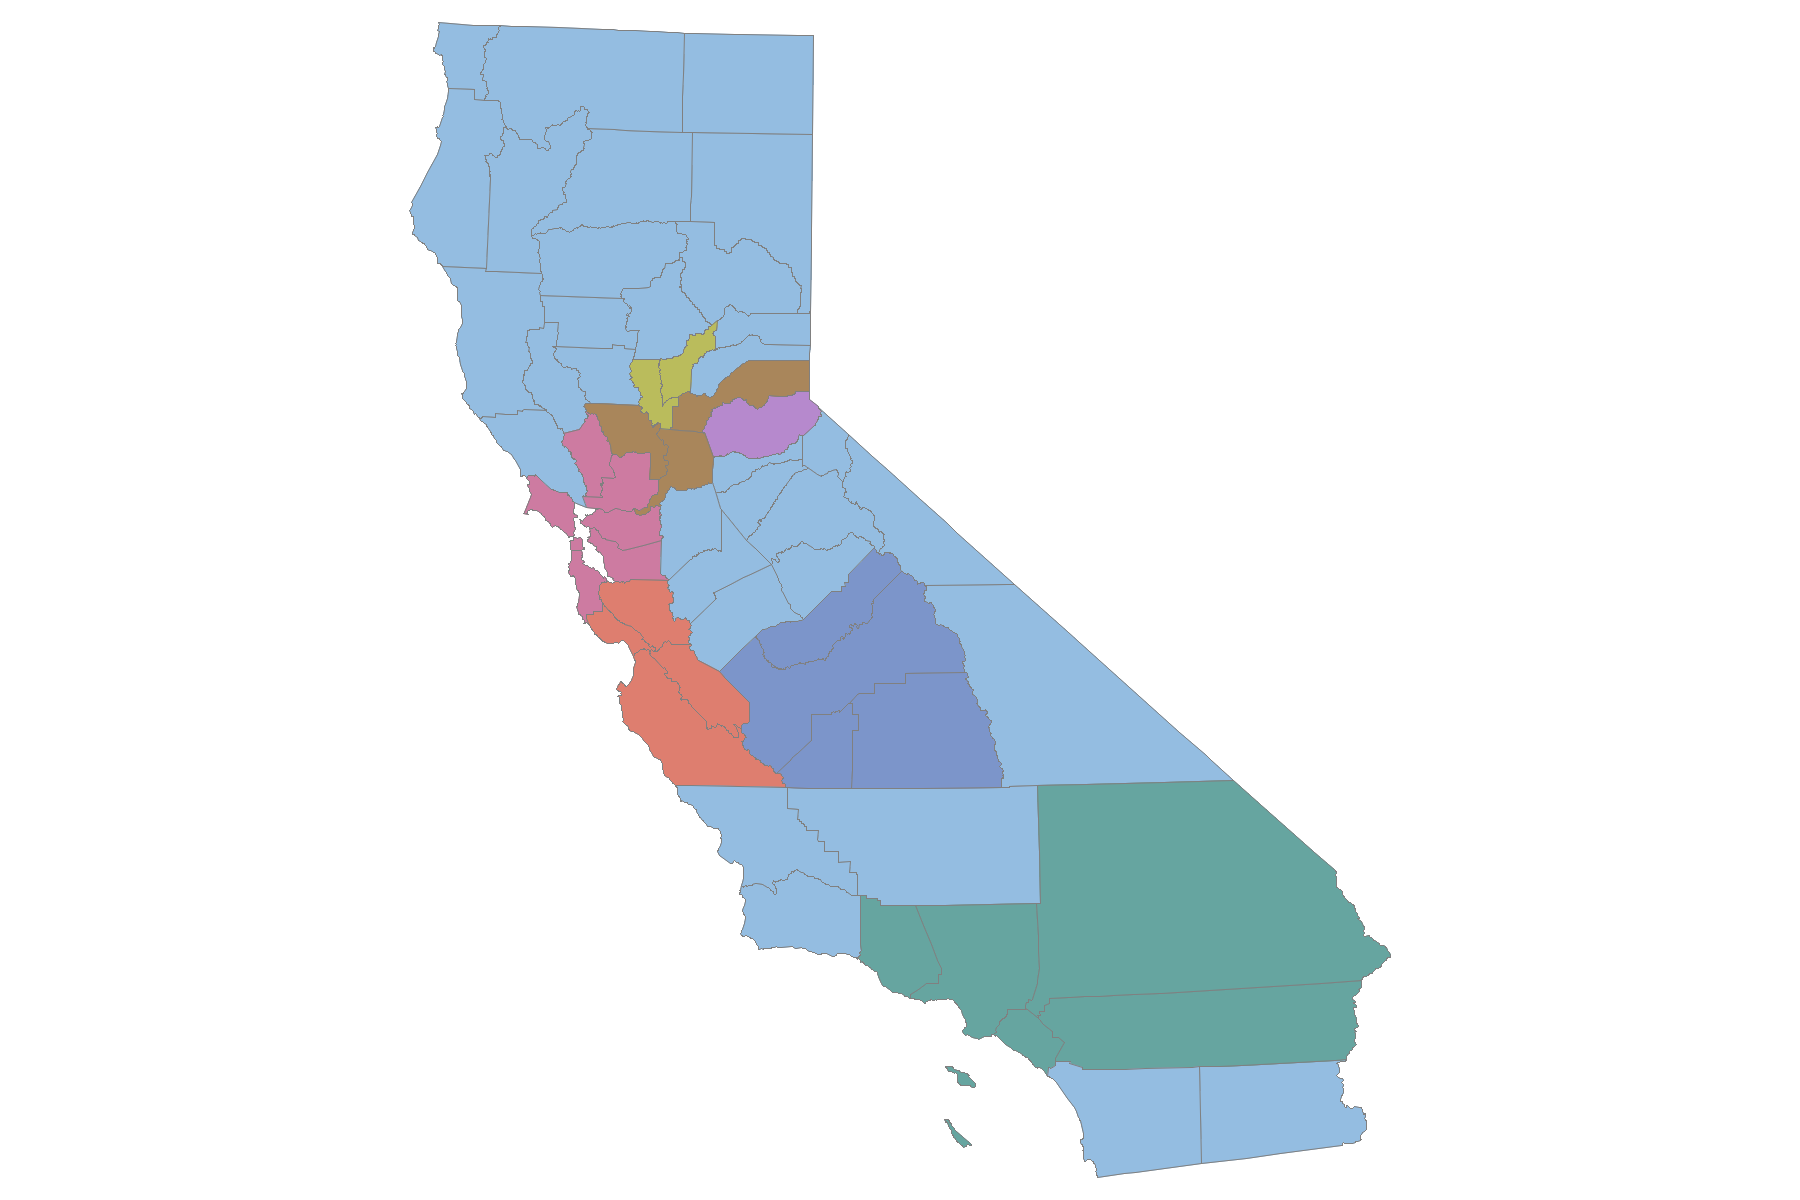
\includegraphics[scale=0.1]{./figures/insetmaps/california_clustermap_960_inset6.png} & 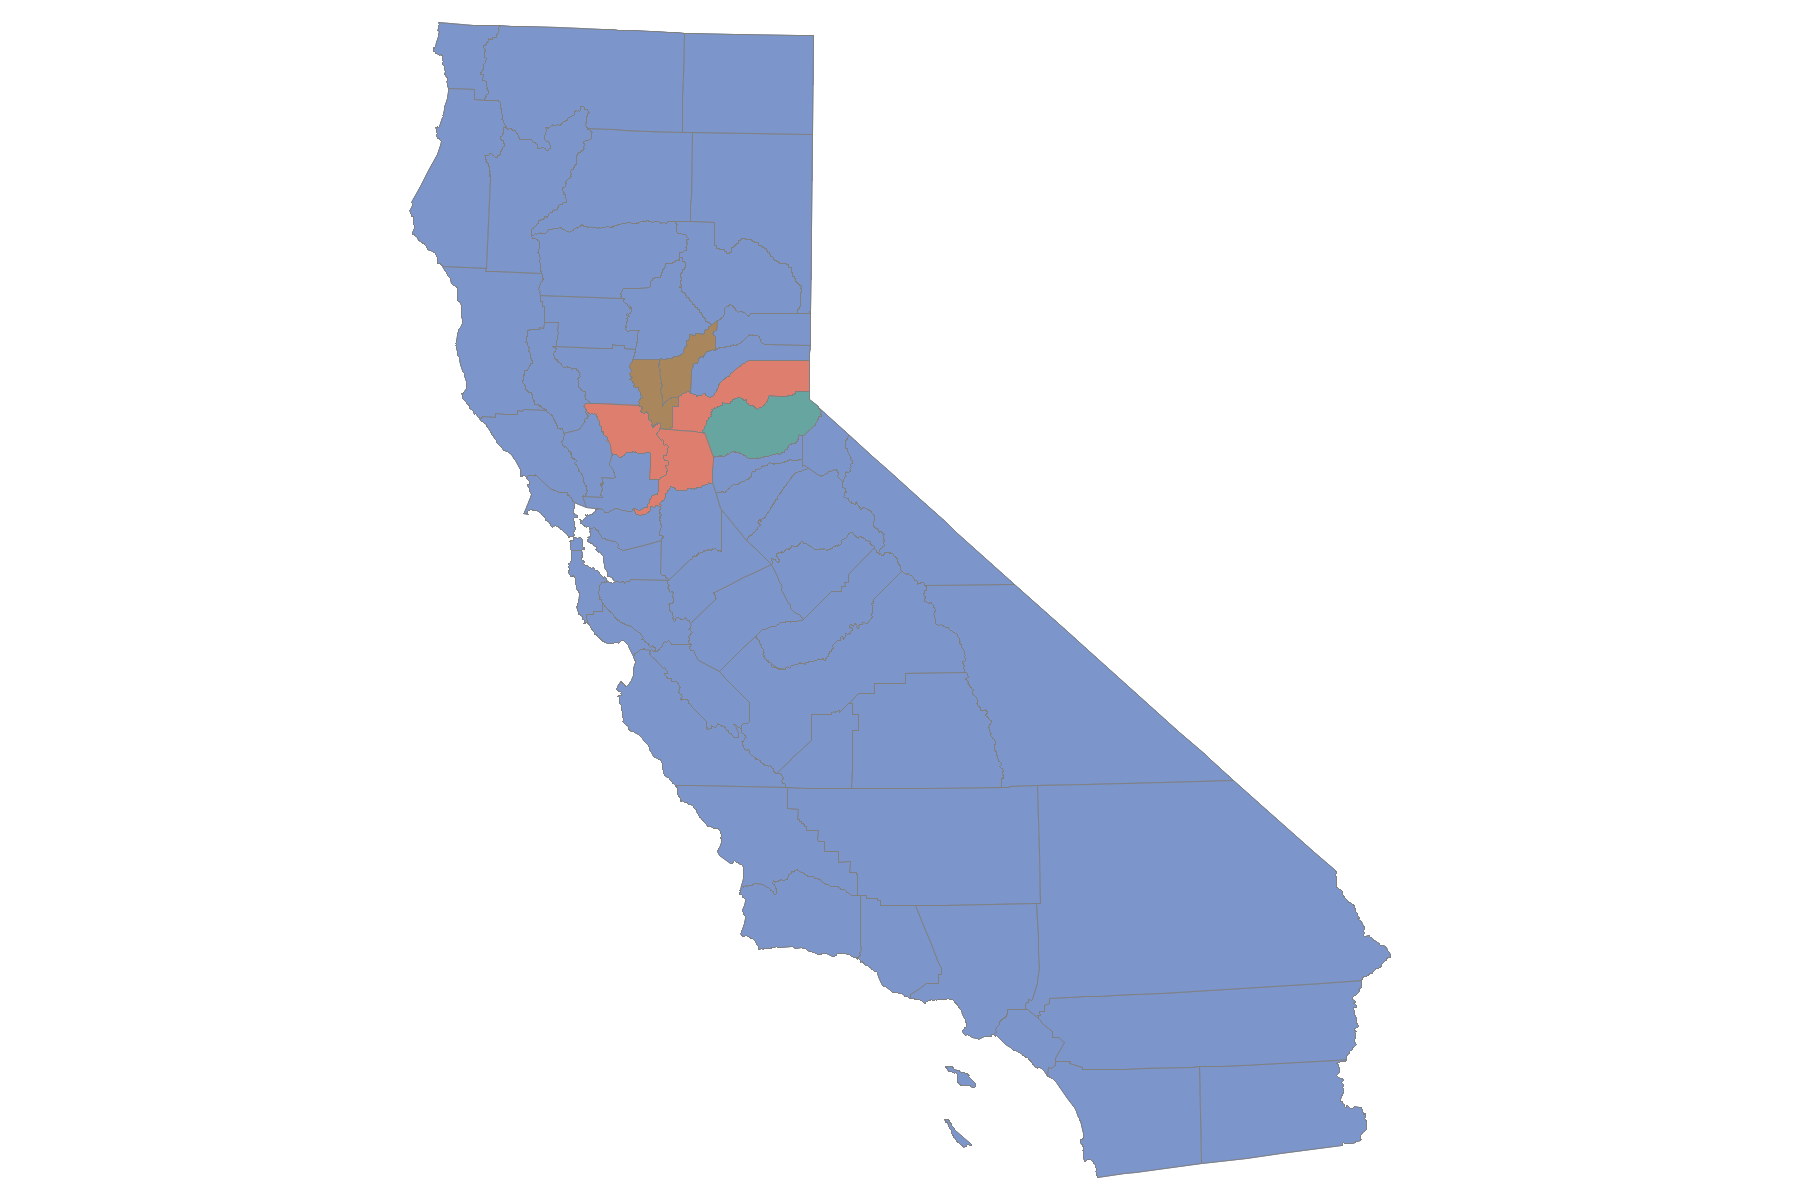
\includegraphics[scale=0.1]{./figures/insetmaps/california_clustermap_1000_inset6.png} \\
Height = 0.96 & Height = 1\\
\multicolumn{2}{p{5in}}{\footnotesize \emph{Notes:} The above graphs are generated using the methodology outlined in Section \ref{sec:method}, using 1990 Census JTW data. More detail is in the text.}
\end{tabular}
\end{figure}

\begin{table}[h]
\caption{Summary Statistics of Ratio of MOE to Flows \label{tab:moesum}}
\begin{tabular}{lcccc}
\hline\hline
& Mean & 25th Pctile & 50th Pctile & 75th Pctile \\
\hline
All counties & 1.236 & 0.845 & 1.370 & 1.600\\
Flows <100 & 1.432 & 1.148 & 1.500 & 1.636 \\
Flows 100-1000 & 0.444 & 0.301 & 0.414 & 0.549  \\
Flows 1000-10000 & 0.131 & 0.087 & 0.124 & 0.169 \\
Flows 10000+ & 0.037 & 0.024 & 0.036 & 0.049 \\
\hline\hline
\multicolumn{5}{p{4in}}{\footnotesize \emph{Notes:} Author's calculation using
2009-2013 ACS Journey-to-Work data.}
\end{tabular}
\end{table}
